\documentclass[]{book}
\usepackage{lmodern}
\usepackage{amssymb,amsmath}
\usepackage{ifxetex,ifluatex}
\usepackage{fixltx2e} % provides \textsubscript
\ifnum 0\ifxetex 1\fi\ifluatex 1\fi=0 % if pdftex
  \usepackage[T1]{fontenc}
  \usepackage[utf8]{inputenc}
\else % if luatex or xelatex
  \ifxetex
    \usepackage{mathspec}
  \else
    \usepackage{fontspec}
  \fi
  \defaultfontfeatures{Ligatures=TeX,Scale=MatchLowercase}
\fi
% use upquote if available, for straight quotes in verbatim environments
\IfFileExists{upquote.sty}{\usepackage{upquote}}{}
% use microtype if available
\IfFileExists{microtype.sty}{%
\usepackage{microtype}
\UseMicrotypeSet[protrusion]{basicmath} % disable protrusion for tt fonts
}{}
\usepackage[margin=1in]{geometry}
\usepackage{hyperref}
\hypersetup{unicode=true,
            pdftitle={Stats 60: Learning stats via simulation},
            pdfauthor={Stats 60 TAs},
            pdfborder={0 0 0},
            breaklinks=true}
\urlstyle{same}  % don't use monospace font for urls
\usepackage{natbib}
\bibliographystyle{apalike}
\usepackage{color}
\usepackage{fancyvrb}
\newcommand{\VerbBar}{|}
\newcommand{\VERB}{\Verb[commandchars=\\\{\}]}
\DefineVerbatimEnvironment{Highlighting}{Verbatim}{commandchars=\\\{\}}
% Add ',fontsize=\small' for more characters per line
\usepackage{framed}
\definecolor{shadecolor}{RGB}{248,248,248}
\newenvironment{Shaded}{\begin{snugshade}}{\end{snugshade}}
\newcommand{\KeywordTok}[1]{\textcolor[rgb]{0.13,0.29,0.53}{\textbf{{#1}}}}
\newcommand{\DataTypeTok}[1]{\textcolor[rgb]{0.13,0.29,0.53}{{#1}}}
\newcommand{\DecValTok}[1]{\textcolor[rgb]{0.00,0.00,0.81}{{#1}}}
\newcommand{\BaseNTok}[1]{\textcolor[rgb]{0.00,0.00,0.81}{{#1}}}
\newcommand{\FloatTok}[1]{\textcolor[rgb]{0.00,0.00,0.81}{{#1}}}
\newcommand{\ConstantTok}[1]{\textcolor[rgb]{0.00,0.00,0.00}{{#1}}}
\newcommand{\CharTok}[1]{\textcolor[rgb]{0.31,0.60,0.02}{{#1}}}
\newcommand{\SpecialCharTok}[1]{\textcolor[rgb]{0.00,0.00,0.00}{{#1}}}
\newcommand{\StringTok}[1]{\textcolor[rgb]{0.31,0.60,0.02}{{#1}}}
\newcommand{\VerbatimStringTok}[1]{\textcolor[rgb]{0.31,0.60,0.02}{{#1}}}
\newcommand{\SpecialStringTok}[1]{\textcolor[rgb]{0.31,0.60,0.02}{{#1}}}
\newcommand{\ImportTok}[1]{{#1}}
\newcommand{\CommentTok}[1]{\textcolor[rgb]{0.56,0.35,0.01}{\textit{{#1}}}}
\newcommand{\DocumentationTok}[1]{\textcolor[rgb]{0.56,0.35,0.01}{\textbf{\textit{{#1}}}}}
\newcommand{\AnnotationTok}[1]{\textcolor[rgb]{0.56,0.35,0.01}{\textbf{\textit{{#1}}}}}
\newcommand{\CommentVarTok}[1]{\textcolor[rgb]{0.56,0.35,0.01}{\textbf{\textit{{#1}}}}}
\newcommand{\OtherTok}[1]{\textcolor[rgb]{0.56,0.35,0.01}{{#1}}}
\newcommand{\FunctionTok}[1]{\textcolor[rgb]{0.00,0.00,0.00}{{#1}}}
\newcommand{\VariableTok}[1]{\textcolor[rgb]{0.00,0.00,0.00}{{#1}}}
\newcommand{\ControlFlowTok}[1]{\textcolor[rgb]{0.13,0.29,0.53}{\textbf{{#1}}}}
\newcommand{\OperatorTok}[1]{\textcolor[rgb]{0.81,0.36,0.00}{\textbf{{#1}}}}
\newcommand{\BuiltInTok}[1]{{#1}}
\newcommand{\ExtensionTok}[1]{{#1}}
\newcommand{\PreprocessorTok}[1]{\textcolor[rgb]{0.56,0.35,0.01}{\textit{{#1}}}}
\newcommand{\AttributeTok}[1]{\textcolor[rgb]{0.77,0.63,0.00}{{#1}}}
\newcommand{\RegionMarkerTok}[1]{{#1}}
\newcommand{\InformationTok}[1]{\textcolor[rgb]{0.56,0.35,0.01}{\textbf{\textit{{#1}}}}}
\newcommand{\WarningTok}[1]{\textcolor[rgb]{0.56,0.35,0.01}{\textbf{\textit{{#1}}}}}
\newcommand{\AlertTok}[1]{\textcolor[rgb]{0.94,0.16,0.16}{{#1}}}
\newcommand{\ErrorTok}[1]{\textcolor[rgb]{0.64,0.00,0.00}{\textbf{{#1}}}}
\newcommand{\NormalTok}[1]{{#1}}
\usepackage{longtable,booktabs}
\usepackage{graphicx,grffile}
\makeatletter
\def\maxwidth{\ifdim\Gin@nat@width>\linewidth\linewidth\else\Gin@nat@width\fi}
\def\maxheight{\ifdim\Gin@nat@height>\textheight\textheight\else\Gin@nat@height\fi}
\makeatother
% Scale images if necessary, so that they will not overflow the page
% margins by default, and it is still possible to overwrite the defaults
% using explicit options in \includegraphics[width, height, ...]{}
\setkeys{Gin}{width=\maxwidth,height=\maxheight,keepaspectratio}
\IfFileExists{parskip.sty}{%
\usepackage{parskip}
}{% else
\setlength{\parindent}{0pt}
\setlength{\parskip}{6pt plus 2pt minus 1pt}
}
\setlength{\emergencystretch}{3em}  % prevent overfull lines
\providecommand{\tightlist}{%
  \setlength{\itemsep}{0pt}\setlength{\parskip}{0pt}}
\setcounter{secnumdepth}{5}
% Redefines (sub)paragraphs to behave more like sections
\ifx\paragraph\undefined\else
\let\oldparagraph\paragraph
\renewcommand{\paragraph}[1]{\oldparagraph{#1}\mbox{}}
\fi
\ifx\subparagraph\undefined\else
\let\oldsubparagraph\subparagraph
\renewcommand{\subparagraph}[1]{\oldsubparagraph{#1}\mbox{}}
\fi

%%% Use protect on footnotes to avoid problems with footnotes in titles
\let\rmarkdownfootnote\footnote%
\def\footnote{\protect\rmarkdownfootnote}

%%% Change title format to be more compact
\usepackage{titling}

% Create subtitle command for use in maketitle
\newcommand{\subtitle}[1]{
  \posttitle{
    \begin{center}\large#1\end{center}
    }
}

\setlength{\droptitle}{-2em}
  \title{Stats 60: Learning stats via simulation}
  \pretitle{\vspace{\droptitle}\centering\huge}
  \posttitle{\par}
  \author{Stats 60 TAs}
  \preauthor{\centering\large\emph}
  \postauthor{\par}
  \predate{\centering\large\emph}
  \postdate{\par}
  \date{2017-01-01}

\usepackage{booktabs}

\begin{document}
\maketitle

{
\setcounter{tocdepth}{1}
\tableofcontents
}
\chapter{Prerequisites}\label{prerequisites}

\chapter{Simulation}\label{simulation}

\chapter{Descriptive statistics and data
vizualization}\label{descriptives}

As an analyst, often our first goal is to \textbf{describe} a data set.
What we mean by ``describe'' here is something like: provide an
efficient represenation of the data that is easy for another person to
understand. Two effective tools for this task are \emph{descriptive
statistics} and \emph{data visualization}. It is important to emphasize
that the task here is to summarize and communicate with other humans,
which means that you need to do more than just figure out how to do the
computations. In his statistics book, ognitive scientist, Dan Navarro,
has a really nice paragraph on the philosophy of descriptive statistics,
so I thought I would include it here:

\begin{quote}
Thus it is no small thing to say that the first task of the statistician
and the scientist is to summarise the data, to find some collection of
numbers that can convey to an audience a sense of what has happened.
This is the job of descriptive statistics, but it's not a job that can
be told solely using the numbers. You are a data analyst, not a
statistical software package. Part of your job is to take these
statistics and turn them into a description. When you analyse data, it
is not sufficient to list off a collection of numbers. Always remember
that what you're really trying to do is communicate with a human
audience. The numbers are important, but they need to be put together
into a meaningful story that your audience can interpret. That means you
need to think about framing. You need to think about context. And you
need to think about the individual events that your statistics are
summarising
\end{quote}

With that framing in mind, let's dive into some common statistical
techniques that we can use to efficiently describe our data.

\section{Measures of central
tendency}\label{measures-of-central-tendency}

Answers the question: Where are the data? What is the long-run average
value of repetitions of the same experiment or data-generating process?

\subsection{Mean}\label{mean}

For a data set, the mean provides information about the ``central
tendency'' or the ``center of mass'' of the data, and is typically
denoted using the symbol \(\bar{x}\). Note that if our data set consists
of random samples from a larger population, we need to be careful to
limit the use of the mean to describe our \emph{sample} since the
population mean ( typically denoted \(\mu\)) is different.

To calculate the mean, we take the sum of each value in our data set and
then divide by the number of data points. In formal notation this looks
like:

\[ \bar{x} = \frac{1}{N} \sum_{i=1}^{N} X_i \]

In R, we can quickly compute the mean using the built-in function
\texttt{mean()}. Here we are using the Iris data set, which comes with
your R installation. The data include a set of measurements in
centimeters of the variables sepal length and width and petal length and
width, respectively, for 50 flowers from each of 3 species of iris. The
species are Iris setosa, versicolor, and virginica.

\begin{Shaded}
\begin{Highlighting}[]
\NormalTok{m_plength <-}\StringTok{ }\KeywordTok{mean}\NormalTok{(d$Petal.Length)}
\NormalTok{m_plength}
\end{Highlighting}
\end{Shaded}

\begin{verbatim}
## [1] 3.758
\end{verbatim}

Note that we could also use our dplyr skills to compute the mean like
this.

\begin{Shaded}
\begin{Highlighting}[]
\NormalTok{d %>%}\StringTok{ }\KeywordTok{summarise}\NormalTok{(}\DataTypeTok{m =} \KeywordTok{mean}\NormalTok{(Petal.Length))}
\end{Highlighting}
\end{Shaded}

\begin{verbatim}
##       m
## 1 3.758
\end{verbatim}

Let's practice our data viz skills and plot the distribution of petal
lengths and include the mean as a vertical dashed line.

\begin{Shaded}
\begin{Highlighting}[]
\NormalTok{d %>%}\StringTok{ }
\StringTok{  }\KeywordTok{ggplot}\NormalTok{(}\KeywordTok{aes}\NormalTok{(}\DataTypeTok{x =} \NormalTok{Petal.Length)) +}
\StringTok{  }\KeywordTok{geom_histogram}\NormalTok{(}\DataTypeTok{alpha =} \FloatTok{0.7}\NormalTok{) +}
\StringTok{  }\KeywordTok{geom_vline}\NormalTok{(}\DataTypeTok{xintercept =} \NormalTok{m_plength, }\DataTypeTok{linetype =} \StringTok{"dashed"}\NormalTok{) +}
\StringTok{  }\KeywordTok{annotate}\NormalTok{(}\DataTypeTok{geom =} \StringTok{"text"}\NormalTok{, }\DataTypeTok{x =} \NormalTok{m_plength +}\StringTok{ }\NormalTok{.}\DecValTok{7}\NormalTok{, }\DataTypeTok{y =} \DecValTok{20}\NormalTok{, }
           \DataTypeTok{label =} \KeywordTok{paste}\NormalTok{(m_plength, }\StringTok{"cm"}\NormalTok{), }\DataTypeTok{size =} \DecValTok{6}\NormalTok{)}
\end{Highlighting}
\end{Shaded}

\begin{center}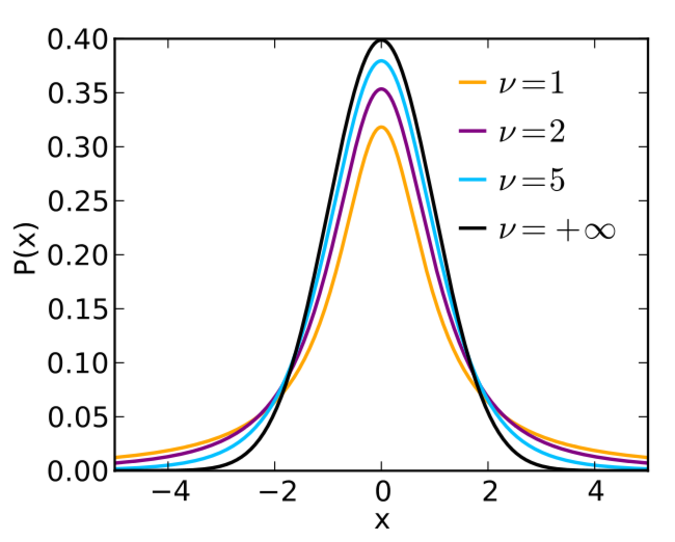
\includegraphics{bookdown-stats60_files/figure-latex/unnamed-chunk-4-1} \end{center}

What do we see? Well, it looks like the mean does tell us about the
center location of these data. One way to think about this is is that
the mean serves as a ``balancig point'' of the data distribution, with
the number to the left of the mean being balanced by the numbers to the
right of the mean.

But, let's return to our original goal of providing a useful description
of these data. Is \texttt{m\_plength} telling us anything useful about
these data? Not really. And if we color our plot based on the species of
iris, we can see what's going on here.

\begin{Shaded}
\begin{Highlighting}[]
\NormalTok{d %>%}\StringTok{ }
\StringTok{  }\KeywordTok{ggplot}\NormalTok{(}\KeywordTok{aes}\NormalTok{(}\DataTypeTok{x =} \NormalTok{Petal.Length, }\DataTypeTok{fill =} \NormalTok{Species)) +}
\StringTok{  }\KeywordTok{geom_density}\NormalTok{(}\DataTypeTok{alpha =} \FloatTok{0.7}\NormalTok{) +}
\StringTok{  }\KeywordTok{theme}\NormalTok{(}\DataTypeTok{legend.position =} \StringTok{"top"}\NormalTok{)}
\end{Highlighting}
\end{Shaded}

\begin{center}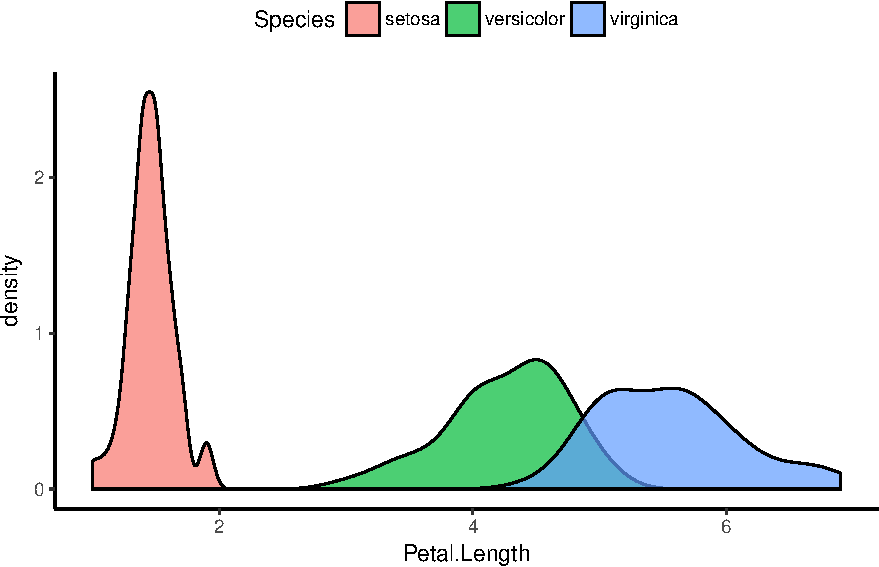
\includegraphics{bookdown-stats60_files/figure-latex/unnamed-chunk-5-1} \end{center}

It looks like there are actually three different distributions of petal
length in our data set. We can use our dplyr skills to compute the mean
for each distribution separately:

\begin{Shaded}
\begin{Highlighting}[]
\NormalTok{ms_petal_length <-}\StringTok{ }\NormalTok{d %>%}\StringTok{ }
\StringTok{  }\KeywordTok{group_by}\NormalTok{(Species) %>%}\StringTok{ }
\StringTok{  }\KeywordTok{summarise}\NormalTok{(}\DataTypeTok{m =} \KeywordTok{mean}\NormalTok{(Petal.Length)) %>%}
\StringTok{  }\KeywordTok{mutate}\NormalTok{(}\DataTypeTok{m =} \KeywordTok{round}\NormalTok{(m, }\DataTypeTok{digits =} \DecValTok{2}\NormalTok{))}
\end{Highlighting}
\end{Shaded}

And add that information to our plot:

\begin{Shaded}
\begin{Highlighting}[]
\NormalTok{d %>%}\StringTok{ }
\StringTok{  }\KeywordTok{ggplot}\NormalTok{(}\KeywordTok{aes}\NormalTok{(}\DataTypeTok{x =} \NormalTok{Petal.Length, }\DataTypeTok{fill =} \NormalTok{Species)) +}
\StringTok{  }\KeywordTok{geom_density}\NormalTok{(}\DataTypeTok{alpha =} \FloatTok{0.7}\NormalTok{) +}
\StringTok{  }\KeywordTok{geom_vline}\NormalTok{(}\KeywordTok{aes}\NormalTok{(}\DataTypeTok{xintercept =} \NormalTok{m), }\DataTypeTok{data =} \NormalTok{ms_petal_length, }\DataTypeTok{linetype =} \StringTok{"dashed"}\NormalTok{, }\DataTypeTok{size =} \DecValTok{1}\NormalTok{) +}
\StringTok{  }\KeywordTok{geom_text}\NormalTok{(}\KeywordTok{aes}\NormalTok{(}\DataTypeTok{label =} \KeywordTok{paste}\NormalTok{(m, }\StringTok{"cm"}\NormalTok{), }\DataTypeTok{x =} \NormalTok{m +}\StringTok{ }\FloatTok{0.6}\NormalTok{, }\DataTypeTok{y =} \DecValTok{2}\NormalTok{), }\DataTypeTok{data =} \NormalTok{ms_petal_length, }\DataTypeTok{size =} \DecValTok{5}\NormalTok{) +}
\StringTok{  }\KeywordTok{theme}\NormalTok{(}\DataTypeTok{legend.position =} \StringTok{"top"}\NormalTok{)}
\end{Highlighting}
\end{Shaded}

\begin{center}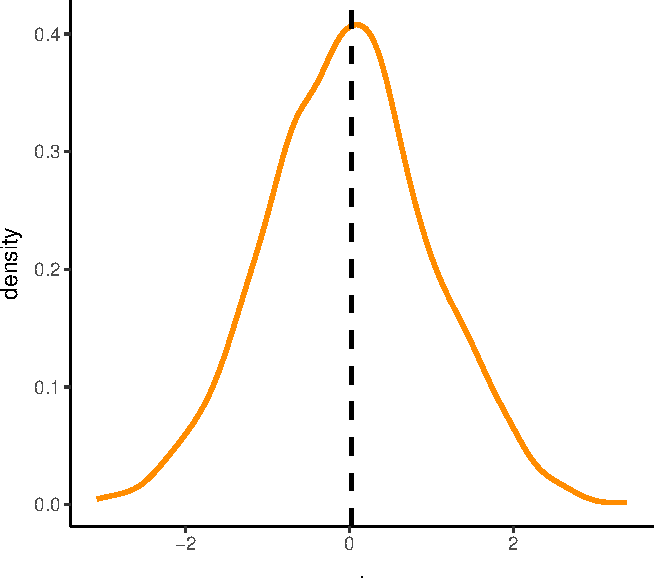
\includegraphics{bookdown-stats60_files/figure-latex/unnamed-chunk-7-1} \end{center}

I would argue that these three numbers -- the mean for each type of iris
species in the data set -- give us a more useful description of the
central tendency. And you can say something like, ``The average petal
length for the setosa species is 1.46.''

\subsection{Median}\label{median}

\subsection{Mode}\label{mode}

\section{Measures of variability}\label{measures-of-variability}

Answers the question: How spread out are the data?

\subsection{Range}\label{range}

\subsection{Interquartile range}\label{interquartile-range}

The interquartile range (IQR) refers to the middle 50\% of a data
distribution. It provides a useful way to describe how spread out the
data are. To compute the IQR, you divide your data into quartiles or
four equal parts. You then subtract the first quartile value from the
third quartil value: \(IQR = Q3 − Q1\)

Things get a little trickier when we are trying to compute the IQR for
continuous-valued distributions. We need to use calculus to integrate
the probability density function to get the cumulative distribution
function (CDF). The CDF provides the following pieces of information:

\begin{itemize}
\tightlist
\item
  The lower quartile, Q1, is a number such that integral of the PDF from
  \(-\infty\) to Q1 equals 0.25
\item
  The upper quartile, Q3, is such a number that the integral from
  \(-\infty\)to Q3 equals 0.75.
\end{itemize}

\subsection{Mean Absolute Deviation}\label{mean-absolute-deviation}

The mean absolute deviation (MAD) is another measure of the amount of
dispersion in your data. Intuitively, it provides a measure of how far
your data are from the mean. Here is the formal definition:

\[MAD = \frac{1}{n} \displaystyle\sum_{i=1}^{n} |x_i - \bar{x}|\]

Really, this formula is just a compact way to describe the following
algorithm:

\begin{enumerate}
\def\labelenumi{\arabic{enumi}.}
\tightlist
\item
  Compute the mean of the sample
\item
  Compute the difference between each data point and the mean
\item
  Add all of those differences
\item
  Divide by the number of data points in the sample
\end{enumerate}

\subsection{Variance}\label{variance}

\[\sigma^2 = \frac{1}{n} \displaystyle\sum_{i=1}^{n} (x_i - \bar{x})^2\]

\subsection{Standard deviation}\label{standard-deviation}

\[\sigma = \sqrt{\frac{1}{n-1} \displaystyle\sum_{i=1}^{n} (x_i - \bar{x})^2}\]

\section{Standard scores}\label{standard-scores}

\chapter{T-test}\label{t-test}

\bibliography{packages.bib,book.bib}


\end{document}
